\subsection{Node-level}

\subsubsection{Server (computation, HW accelerators)}\label{subsubsection: Server (computation, HW accelerators)}

\definition{Server}s are like ordinary PCs, usually more powerful, but with a \textbf{form factor that allows them to fit into the shelves} (such as rack, blade enclosure format, or tower; the differences are explained later). They are usually built in a tray or blade enclosure format, \textbf{housing the motherboard}, the \textbf{chipset}, and \textbf{additional plug-in components}.

\highspace
The \textbf{motherboard} acts as the central hub, \textbf{connecting all the crucial components of the server and enabling them to communicate and work together}.

It provides sockets and plug-in slots to install CPUs, memory modules (DIMMs), local storage (such as Flash SSDs or HDDs), and network interface cards (NICs) to satisfy the range of resource requirements.

\highspace
The \textbf{chipsets} and \textbf{additional components} are grouped in the following way:
\begin{itemize}
    \item Number and type of CPUs:
    \begin{itemize}
        \item From 1 to 8 CPU socket.
        \item Intel Xeon Family, AMD EPYC, etc.
    \end{itemize}

    \item Available RAM:
    \begin{itemize}
        \item From 2 to 192 DIMM Slots.
    \end{itemize}

    \item Locally attached disks:
    \begin{itemize}
        \item From 1 to 24 Drive Bays. 
        \item HDD or SSD.
        \item SAS (higher performance but more expensive) or SATA (for entry-level servers).
    \end{itemize}

    \item Other special purpose devices:
    \begin{itemize}
        \item From 1 to 20 GPUs per node, or TPUs.
        \item NVIDIA Pascal, Volta, etc.
    \end{itemize}
    
    \item Form factor:
    \begin{itemize}
        \item From 1 unit to 10 units.
        \item Tower.
    \end{itemize}
\end{itemize}

\newpage

\begin{center}
    \textcolor{Red2}{\textbf{Differences between Rack, Blade and Tower}}
\end{center}

\subsubsection*{Tower Server}

A \definition{Tower Server} looks and feels much like a \textbf{traditional} tower \textbf{PC}.

\begin{flushleft}
    \textcolor{Green3}{\faIcon{check} \textbf{Advantages}}
\end{flushleft}
\begin{itemize}[label=\ding{51}]
    \item \textbf{Scalability} and \textbf{ease of upgrade}. Customized and upgraded based on necessity.

    \item \textbf{Cost-effective}. Tower servers are probably the \emph{cheapest of all kinds of servers}.

    \item \textbf{Cools easily}. Since a tower server has a low overall component density, it cools down easily.
\end{itemize}

\begin{flushleft}
    \textcolor{Red2}{\faIcon{thumbs-down} \textbf{Disadvantages}}
\end{flushleft}
\begin{itemize}[label=\ding{55}]
    \item \textbf{Consumes a lot of space}. These servers are difficult to manage physically.

    \item \textbf{Provides a basic level of performance}. A tower server is \emph{ideal for small business that have a limited number of clients}.

    \item \textbf{Complicated cable management}. Devices aren't easily routed together.
\end{itemize}

\newpage

\paragraph{Rack Servers}

\definition{Rack Servers} are unique \textbf{shelves that accommodate all the IT equipment} and allow their interconnection. The racks are used to store these rack servers.

\highspace
Server racks are measured in \definition{Rack Units}, or "U". One U is approximately 44.45 millimeters. The \underline{main advantage} of these racks is that they \textbf{allow designers to stack up other electronic devices and servers}.

\highspace
A rack server is designed to be positioned in a bay by vertically stacking servers one over the other along with other devices (storage units, cooling systems, network peripherals, and batteries).

\begin{flushleft}
    \textcolor{Green3}{\faIcon{check} \textbf{Advantages}}
\end{flushleft}
\begin{itemize}[label=\ding{51}]
    \item \textbf{Failure containment}. Very little effort to identify, remove, and replace a malfunctioning server with another.

    \item \textbf{Simplified cable management}. Easy and efficient to organize cables.

    \item \textbf{Cost-effective}. Computing power and efficiency at relatively lower costs.
\end{itemize}

\begin{flushleft}
    \textcolor{Red2}{\faIcon{thumbs-down} \textbf{Disadvantages}}
\end{flushleft}
\begin{itemize}[label=\ding{55}]
    \item \textbf{Power usage}. Needs of additional cooling systems due to their high overall component density, thus consuming more power.

    \item \textbf{Maintenance}. Since multiple devices are placed in racks together, maintaining them gets considerably though with the increasing number of racks.
\end{itemize}

\newpage

\paragraph{Blade Servers}

\definition{Blade Servers} are the latest and the most advanced type of servers in the market. They can be termed hybrid rack servers, where servers are placed inside blade enclosures, forming a blade system.

\highspace
The \textbf{most significant advantage} of blade servers is that these servers are the \textbf{most minor types of servers available now} and are \textbf{great for conserving space}.

\highspace
Finally, a blade system also meets the IEEE standard for rack units, and each rack is measured in the units of "U".

\begin{flushleft}
    \textcolor{Green3}{\faIcon{check} \textbf{Advantages}}
\end{flushleft}
\begin{itemize}[label=\ding{51}]
    \item \textbf{Size and form factor}. They are smallest and the most compact servers, requiring minimal physical space. Blade servers offer \emph{higher space efficiency} compared to traditional rack-mounted servers.

    \item \textbf{Cabling}. Blade server don't involve the cumbersome tasks of setting up cabling. Although you still might have to deal with the cabling, it is near to negligible when compared to tower and rack servers.

    \item \textbf{Centralized management}. Blade enclosures typically come with centralized management tools that allow administrators to easily monitor, configure and update all blades from a single interface.

    \item \textbf{Load balancing, failover, scalability}. Uniform system, shared components (including network), simple addition/removal of servers.
\end{itemize}

\begin{flushleft}
    \textcolor{Red2}{\faIcon{thumbs-down} \textbf{Disadvantages}}
\end{flushleft}
\begin{itemize}[label=\ding{55}]
    \item \textbf{Expensive configuration and Higher initial cost}. Although upgrading the blade server is easy to handle and manage, the initial configuration or the setup requires more effort and higher initial investment.

    \item \textbf{Vendor Lock-In}. Blade servers typically require the use of the manufacturer's specific blades and enclosures, leading to vendor lock-in. This can limit flexibility and potentially increase costs in the long run.

    \item \textbf{Cooling}. Blade servers come with high component density. Therefore, special accommodations have to be arranged for these servers to ensure they don't get overheated. Heating, ventilation, and air conditioning systems (HVAC) must be carefully managed and designed.
\end{itemize}

\newpage

\paragraph{Machine Learning}

\begin{deepeningbox}[: Machine Learning (supervised learning)]
    \textbf{Machine learning} (ML) is a branch of artificial intelligence (AI) and computer science that focuses on the using data and algorithms to enable AI to imitate the way that humans learn, gradually improving its accuracy (\href{https://www.ibm.com/topics/machine-learning}{source}).

    \highspace
    \href{https://ischoolonline.berkeley.edu/blog/what-is-machine-learning/}{UC Berkeley} breaks out the learning system of a machine learning algorithm into three main parts:
    \begin{enumerate}
        \item A Decision Process: In general, machine learning algorithms are used to make a prediction or classification. Based on some input data, which can be labeled or unlabeled, your algorithm will produce an estimate about a pattern in the data.

        \item An Error Function: An error function evaluates the prediction of the model. If there are known examples, an error function can make a comparison to assess the accuracy of the model.

        \item A Model Optimization Process: If the model can fit better to the data points in the training set, then weights are adjusted to reduce the discrepancy between the known example and the model estimate. The algorithm will repeat this iterative \dquotes{evaluate and optimize} process, updating weights autonomously until a threshold of accuracy has been met.
    \end{enumerate}

    \highspace
    The main goal is to learn a target function that can be used for prediction. Given a training set of labeled examples $\left\{\left(x_{1}, y_{1}\right), \dots, \left(x_{n}, y_{n}\right)\right\}$, estimate the prediction function $f$ by minimizing the prediction error on the training set:
    \begin{equation*}
        y = f\left(x\right)
    \end{equation*}
    Where $y$ is the output, $f$ is the prediction function and the $x$ is an image feature.
\end{deepeningbox}

\begin{deepeningbox}[: Artificial Neural Network]
    The \textbf{Artificial Neural Network} is a computational model inspired by the human brain (perceptron). It consists of interconnected nodes (neurons) organized in layers to process and analyze data and used to learn data representation from data (learn features and the classifier/regressor).

    \highspace
    The learning process of a Neural Network is as follows: Neurons make decisions (activation functions). There are wights, so the connections between neurons are strengthened or weakened through training- randomly initialized.

    The (training data) Neural Networks learn from historical data and examples. Then, labeled data are provided.
\end{deepeningbox}

\begin{deepeningbox}[: effects of ML and ANN]
    Deep learning models began to appear and be widely adopted, enabling specialized hardware to power a broad spectrum of machine learning solutions.
    
    Since 2013, AI learning compute requirements have doubled every 3.5 months (vs. 18-24 months expected from \href{https://en.wikipedia.org/wiki/Moore's_law}{Moore's Law}).

    To satisfy the growing compute needs for deep learning, \textbf{WSCs deploy specialized accelerator hardware}:
    \begin{itemize}
        \item Graphical Processing Units (GPUs) are used for data-parallel computations (the same program is executed on many data elements in parallel). In order to use parallel programming, high-level languages such as CUDA, OpenCL, OPENACC, OpenMP, and SYCL exist. This technique allows up to 1000x faster than CPU.


        \item Tensor Processing Unit (TPU), where Tensor is a n-dimensional matrix, are used for training and inference.


        \item Field-Programmable Gate Array (FPGA) are programmable hardware devices. The device user can program an array of logic gates (\dquotes{configured}) in the field instead of the people who designed it. An array of carefully designed and interconnected digital subcircuits that efficiently implement common functions, offering very high levels of flexibility. The digital subcircuits are called configurable logic blocks (CLBs).

        FPGA Applications in Data Centers:
        \begin{itemize}
            \item Network acceleration: FPGAs can offload specific processing tasks from CPUs, improving overall network performance and reducing CPU workload.

            \item Security acceleration: Encryption, decryption, and other security-related tasks can be accelerated using FPGAs, enhancing data centre security while maintaining performance.

            \item Data analytics: FPGAs can accelerate specific algorithms in data analytics workloads, leading to faster data processing and analysis.

            \item Machine learning: FPGAs can be configured to efficiently implement specific machine learning algorithms, potentially offering performance advantages for specialized tasks.
        \end{itemize}
    \end{itemize}
\end{deepeningbox}

\newpage

\begin{table}[!htp]
    \centering
    \begin{tabular}{@{} c p{14em} p{14em} @{}}
        \toprule
        & \textbf{Advantages} & \textbf{Disadvantages} \\
        \midrule
        \textbf{CPU} & 
        \begin{itemize}
            \item Easy to be programmed and support any programming framework.
            \item Fast design space exploration and run your applications.
        \end{itemize}
        & \begin{itemize}
            \item Suited only for simple AI models that do not take long to train and for small models with small training set.
        \end{itemize} \\
        \cmidrule{1-3}
        %
        \textbf{GPU} & \begin{itemize}
            \item Ideal for applications in which data need to be processed in parallel like the pixels of images or videos.
        \end{itemize} & \begin{itemize}
            \item Programmed in languages like CUDA and OpenCL and therefore provide limited flexibility compared to CPUs.
        \end{itemize} \\
        \cmidrule{1-3}
        %
        \textbf{TPU} & \begin{itemize}
            \item Very fast at performing dense vector and matrix computations and are specialized on running very fast programming based on Tensorflow.
        \end{itemize} & \begin{itemize}
            \item For applications and models based on the TensorFlow.
            \item Lower flexibility compared to CPUs and GPUs.
        \end{itemize} \\
        \cmidrule{1-3}
        %
        \textbf{FPGA} & \begin{itemize}
            \item Higher performance, lower cost and lower power consumption compared to other options like CPUs and GPU.
        \end{itemize} & \begin{itemize}
            \item Programmed using OpenCL and High-Level Synthesis (HLS).
            \item Limited flexibility compared to other platforms.
        \end{itemize} \\
        \bottomrule
    \end{tabular}
\end{table}

\newpage

\subsubsection{Storage (type, technology)}\label{subsubsection: Storage (type, technology)}

Data has significantly grown in the last few years due to sensors, industry 4.0, AI, etc. The growth favours the \textbf{centralized storage strategy} that is focused on the following:
\begin{itemize}
    \item \textbf{Limiting redundant data}
    \item \textbf{Automatizing replication and backup}
    \item \textbf{Reducing management costs}
\end{itemize}

\highspace
The \emph{storage technologies} are many. One of the oldest but still used is the \definition{hard disk drive (HDD)}, a magnetic disk with mechanical interactions. Due to its mechanical movement, the \definition{solid-state drive (SSD)} is the best solution (quality-price) because there are no mechanical or moving parts, and they are built out of transistors (NADN flash-based devices). The \definition{non-volatile memory express (NVMe)} also exists, which is the \textbf{latest industry standard} for running PCIe\footnote{\definition{PCIe (peripheral component interconnect express)}. is an interface standard for connecting high-speed components} SSDs.

\highspace
As for price classification, we can see that the NVMe is the most expensive solution:
\begin{enumerate}
    \item NVMe (between 100€ and 200€ for 1TB)
    \item SSD (between 70€ and 100€ for 1TB)
    \item HDD (between 40€ and 60€ for 1TB)
\end{enumerate}
For these reasons, it is reasonable to use a \textbf{hybrid solution} (HDD + SSD):
\begin{itemize}
    \item A speed storage technology (\textbf{SSD or NVMe}) as \textbf{cache} and \textbf{several HDDs for storage}. It is a combination used by some servers: a small SSD with a large HDD to have a faster disk.
    
    \item Some HDD manufacturers produce Solid State Hybrid Disks (SSHD) that combine a small SDD with a large HDD in a single unit.
\end{itemize}

\newpage

\paragraph{Files}

An \textbf{OS can see the disks as a collection of} \definition{data blocks} that can be read or written independently. To allow the ordering/management among them, \textbf{each block is characterized by a unique numerical address} called \definition{LBA (Logical Block Address)}. Typically, the \textbf{OS groups blocks into clusters}\footnote{\definition{Clusters} are the minimal units an OS can read from or write to a disk.} \textbf{to simplify the access to the disk}. Typical cluster sizes range from 1 disk sector (512 B, or 4 KB) to 128 sectors (64 KB).

\highspace
Each \emph{cluster} contains:
\begin{itemize}
    \item \textbf{File data}. The actual content of the files.
    
    \item \textbf{Metadata}. The information required to support the file system:
    \begin{itemize}
        \item File names
        \item Directory structures and symbolic links
        \item Creation, modification, and last access dates
        \item Security information (owners, access list, encryption)
        \item \textbf{Links to the LBA where the file content can be located on the disk}
    \end{itemize}
\end{itemize}
The disk can thus contain \textbf{several types of clusters}:
\begin{itemize}
    \item Metadata:
    \begin{itemize}
        \item Fixed position (to bootstrap the entire file system)
        \item Variable position (to hold the folder structure)
    \end{itemize}
    
    \item File data (the actual content of the files)
    
    \item Unused space (available to contain new files and folders)
\end{itemize}

\begin{figure}[!htp]
    \centering
    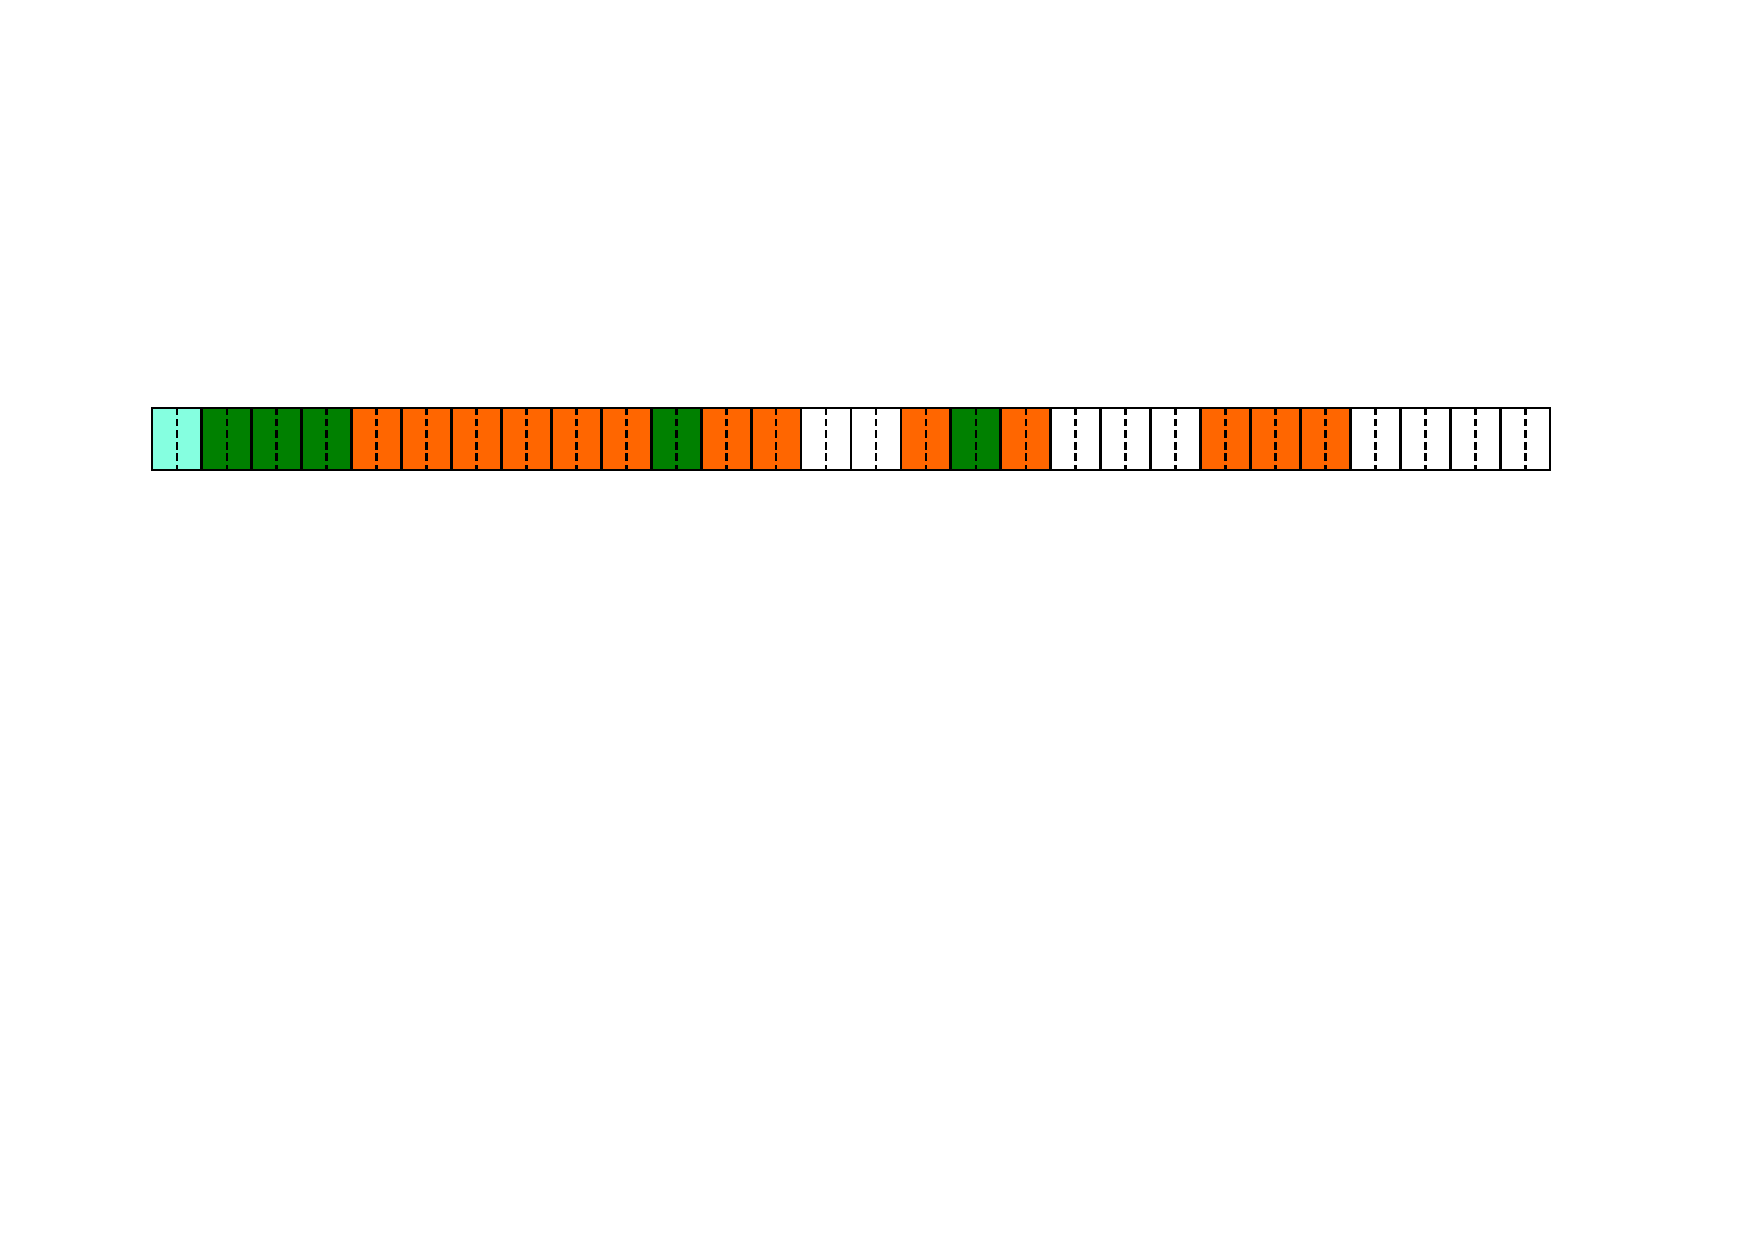
\includegraphics[width=\textwidth]{img/files-1.pdf}
    \caption{A cluster can be seen visually as an array. In this image, for example, we've shown three types of cluster: metadata fixed position (azure), metadata variable position (green), file data (orange), unused space (white).}
\end{figure}

\newpage

\noindent
The following explanation introduces some basic operations on the files to see what happens inside the disks.
\begin{itemize}
    \item \underline{\textbf{Reading}}. To read a file:
    \begin{enumerate}
        \item Access the metadata, variable position (because it contains the folder structure), to locate its block;
        \item Access the blocks to read the contents of the file.
    \end{enumerate}
    \begin{figure}[!htp]
        \centering
        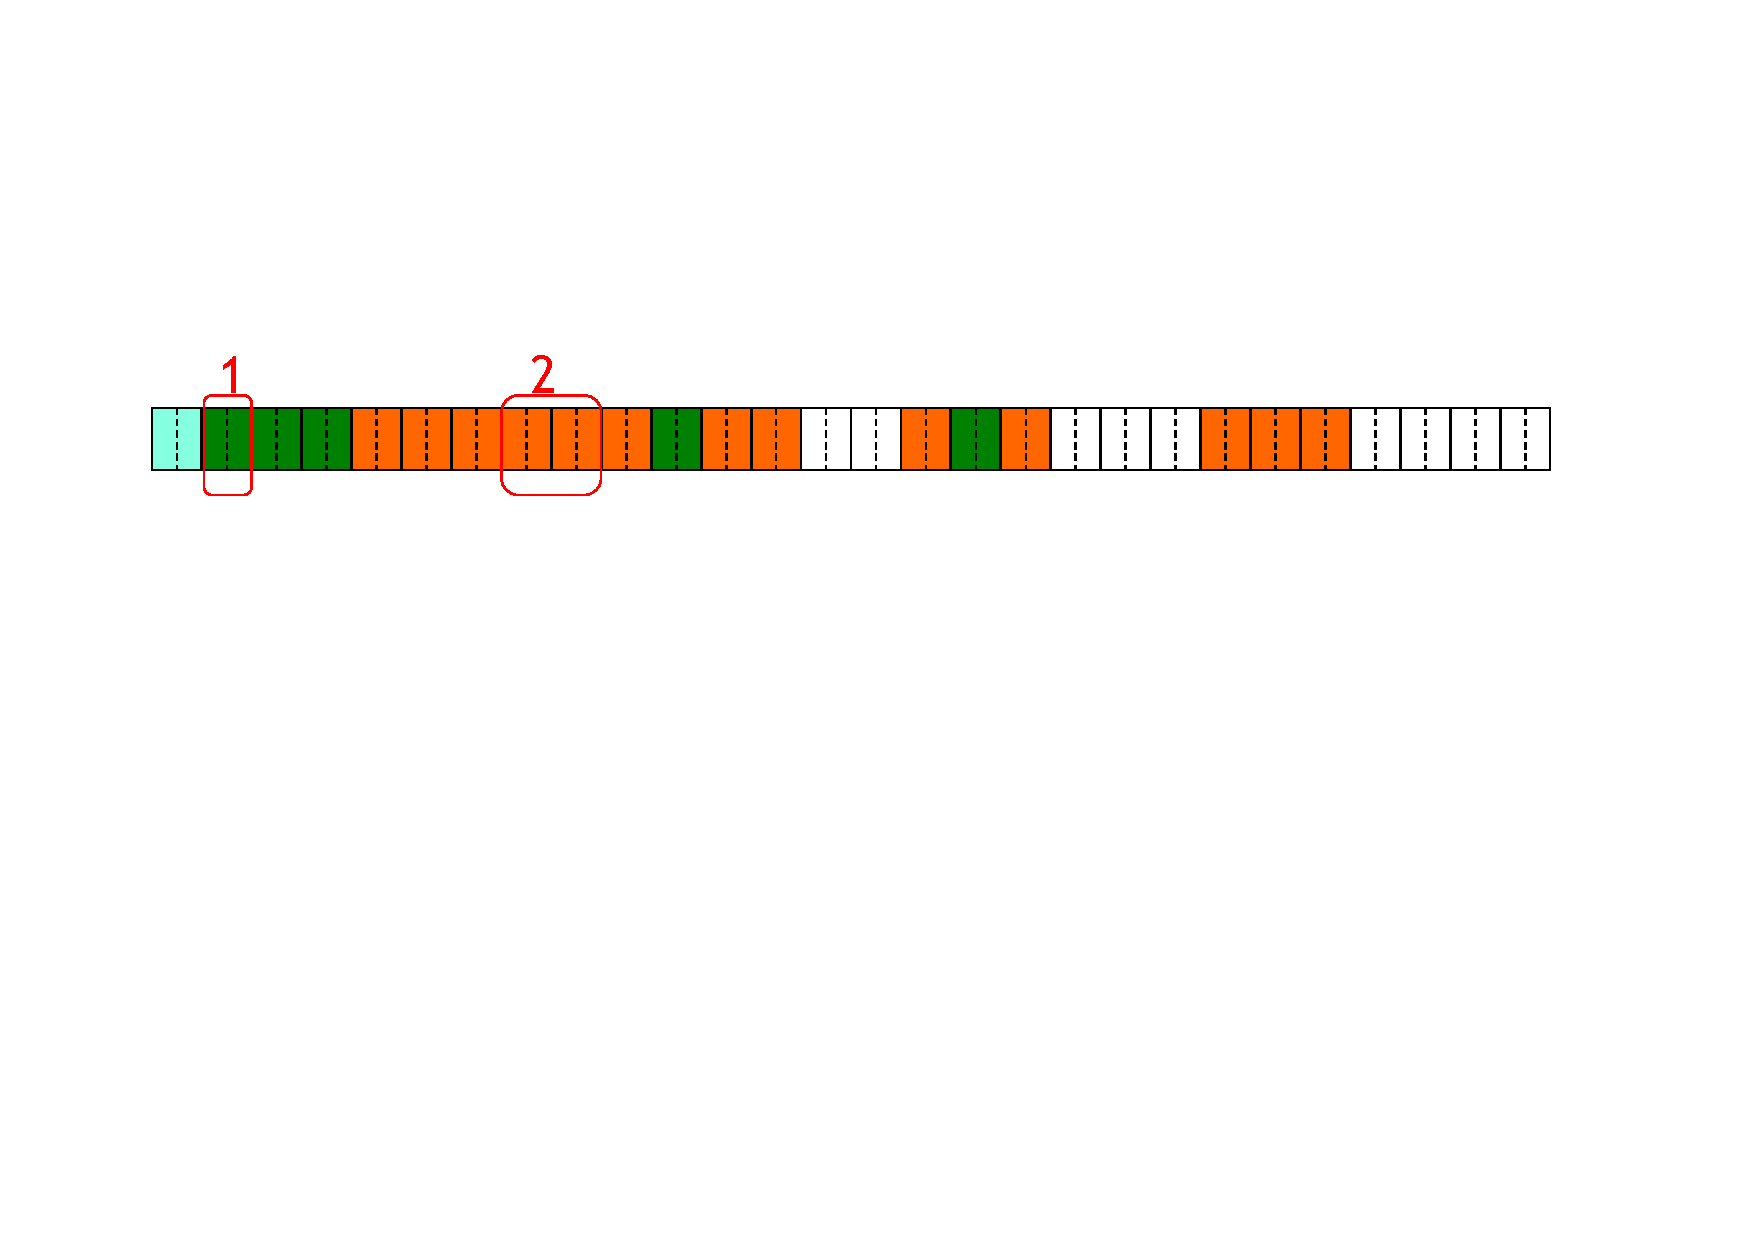
\includegraphics[width=\textwidth]{img/files-2.pdf}
    \end{figure}

    \item \underline{\textbf{Writing}}. To write a file:
    \begin{enumerate}
        \item Access the metadata, variable position (because it contains the folder structure), to find free space.
        \item Write the data in the allocated blocks (cluster type: unused space).        
    \end{enumerate}
    \begin{figure}[!htp]
        \centering
        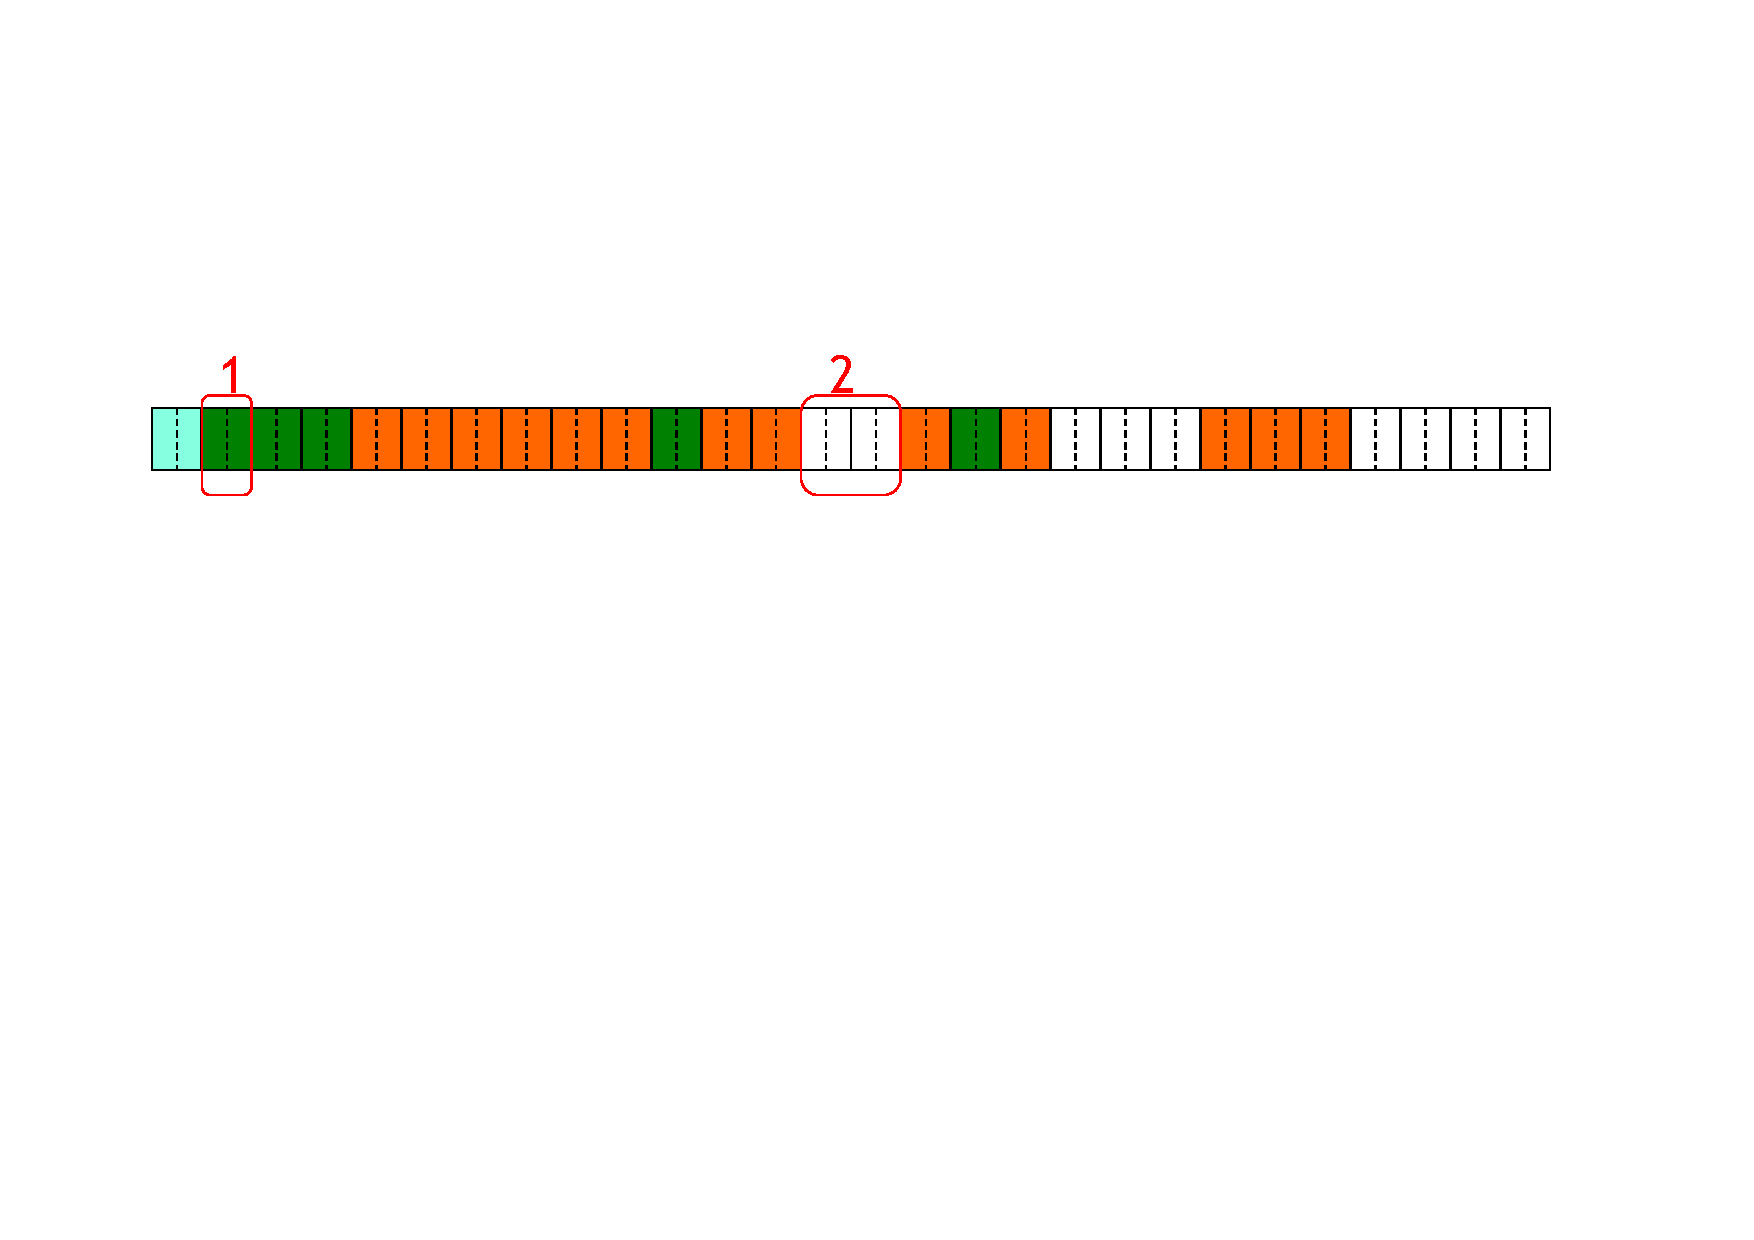
\includegraphics[width=\textwidth]{img/files-3.pdf}
    \end{figure}

    Since the \emph{file system can only access clusters}, the \textbf{actual space taken up by a file on a disk is always a multiple of the cluster size}. Given:
    \begin{itemize}
        \item $s$, the \emph{file size}
        \item $c$, the \emph{cluster size}
    \end{itemize}
    Then the \definition{actual size on the disk $a$} can be calculated as:
    \begin{equation}
        a = \mathrm{ceil}\left(\dfrac{s}{c}\right) \times c
    \end{equation}
    Where $\mathrm{ceil}$ rounds a number \underline{up} to the nearest integer. It's also possible to calculate the \textbf{amount of disk space wasted by organising the file into clusters} (\definition{wasted disk space $w$}):
    \begin{equation}
        w = a - s
    \end{equation}
    A formal way to refer to wasted disk space is \definition{internal fragmentation} of files.
    \newpage
    \begin{examplebox}[: internal fragmentation]
        \begin{itemize}
            \item File size: 27 byte
            \item Cluster size: 8 byte
        \end{itemize}
        The \emph{actual size} on the disk is:
        \begin{equation*}
            a = \mathrm{ceil}\left(\dfrac{27}{8}\right) \cdot 8 = \mathrm{ceil}\left(3.375\right) \cdot 8 = 4 \cdot 8 = 32 \text{ byte}
        \end{equation*}
        And the internal fragmentation $w$ is:
        \begin{equation*}
            w = 32 - 27 = 5 \text{ byte}
        \end{equation*}
    \end{examplebox}

    \item \underline{\textbf{Deleting}}. To delete a file:
    \begin{enumerate}
        \item Just update the metadata, variable position (because it contains the folder structure), to say that the blocks where the file was stored are no longer used by the OS.
    \end{enumerate}
    \textbf{Deleting a file never actually deletes the data on the disk}: if a new file is written to the same clusters, the old data is replaced by the new.
    \begin{figure}[!htp]
        \centering
        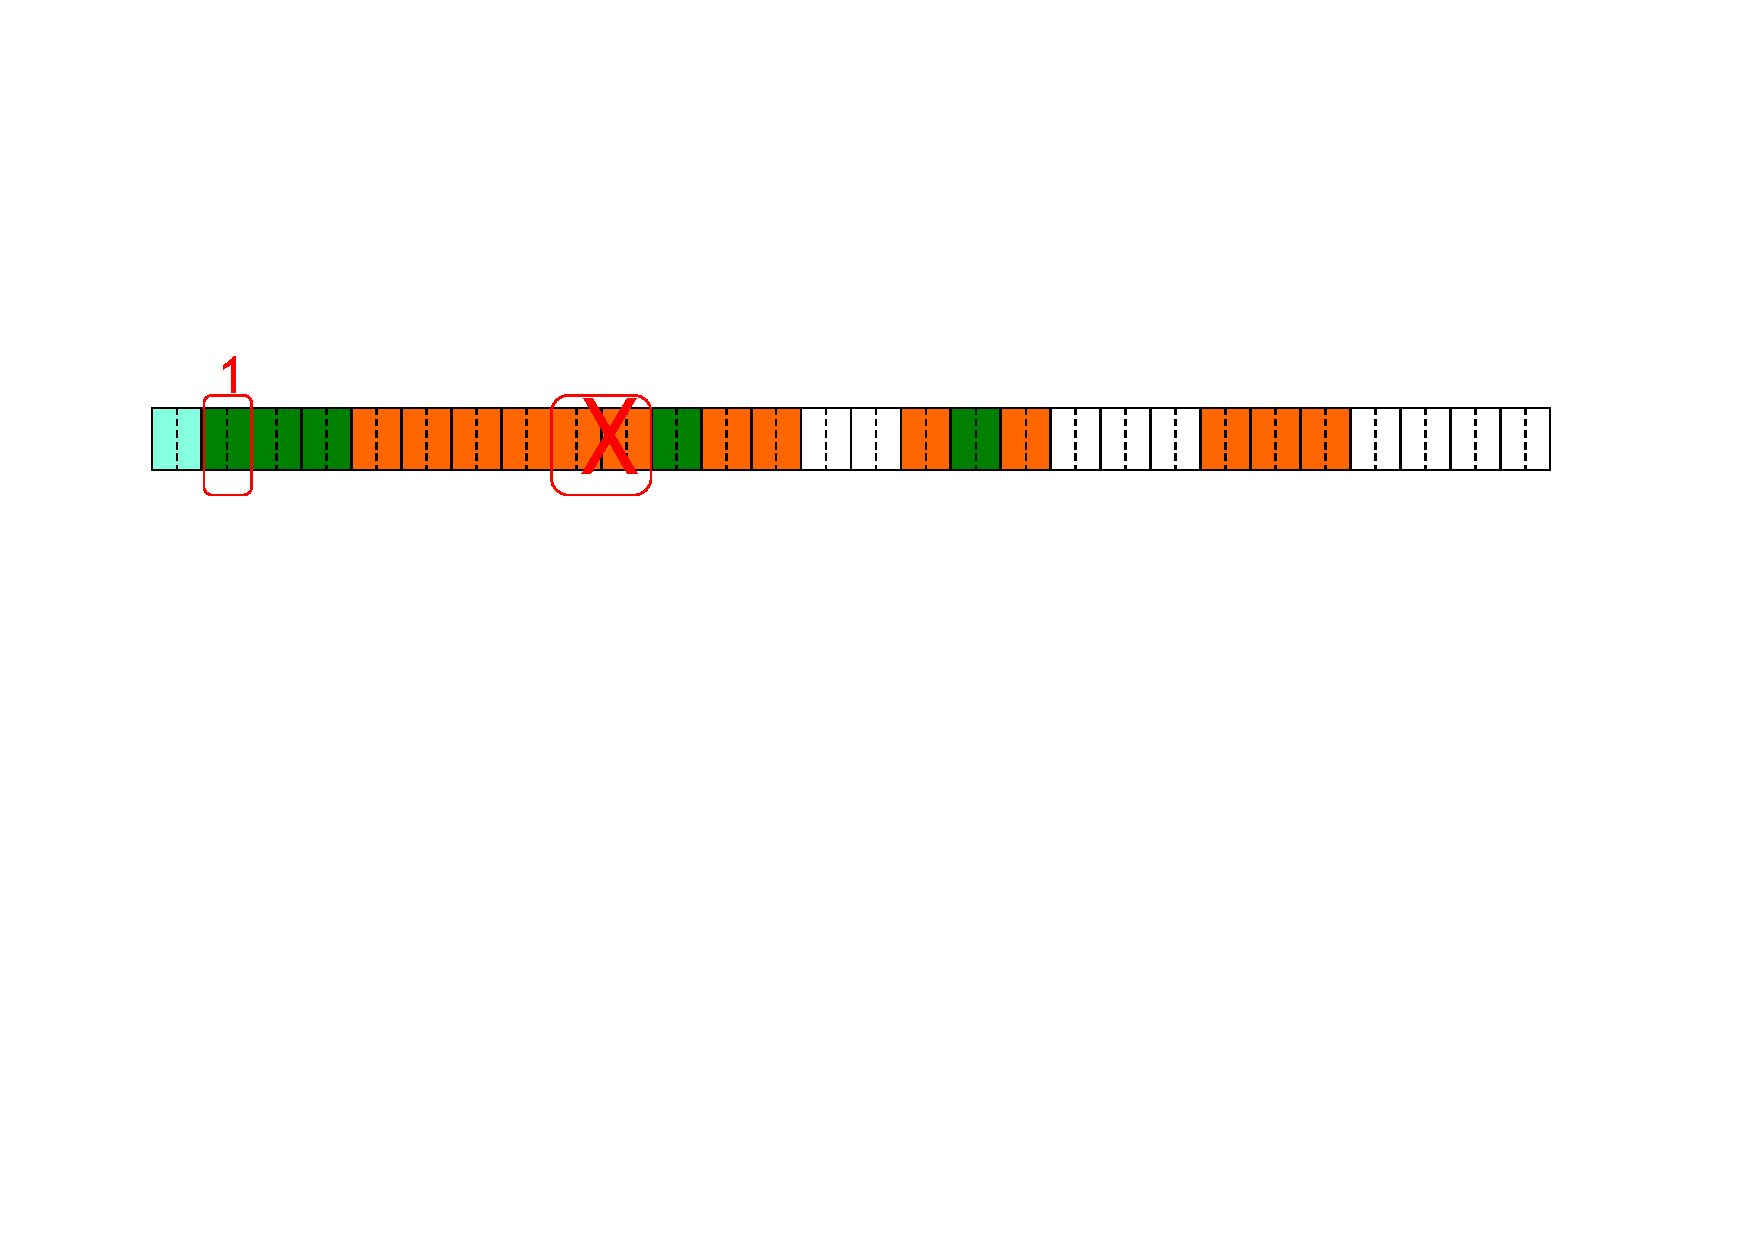
\includegraphics[width=\textwidth]{img/files-4.pdf}
    \end{figure}
    
    \item \underline{\textbf{External fragmentation}}. As the disk's life evolves, there might \textbf{not be enough space to store a file contiguously}.
    
    In this case, the file is split into smaller chunks and inserted into the free clusters spread over the disk.
    
    The effect of \textbf{splitting a file into non-contiguous clusters} is called \definition{external fragmentation}.
    \begin{figure}[!htp]
        \centering
        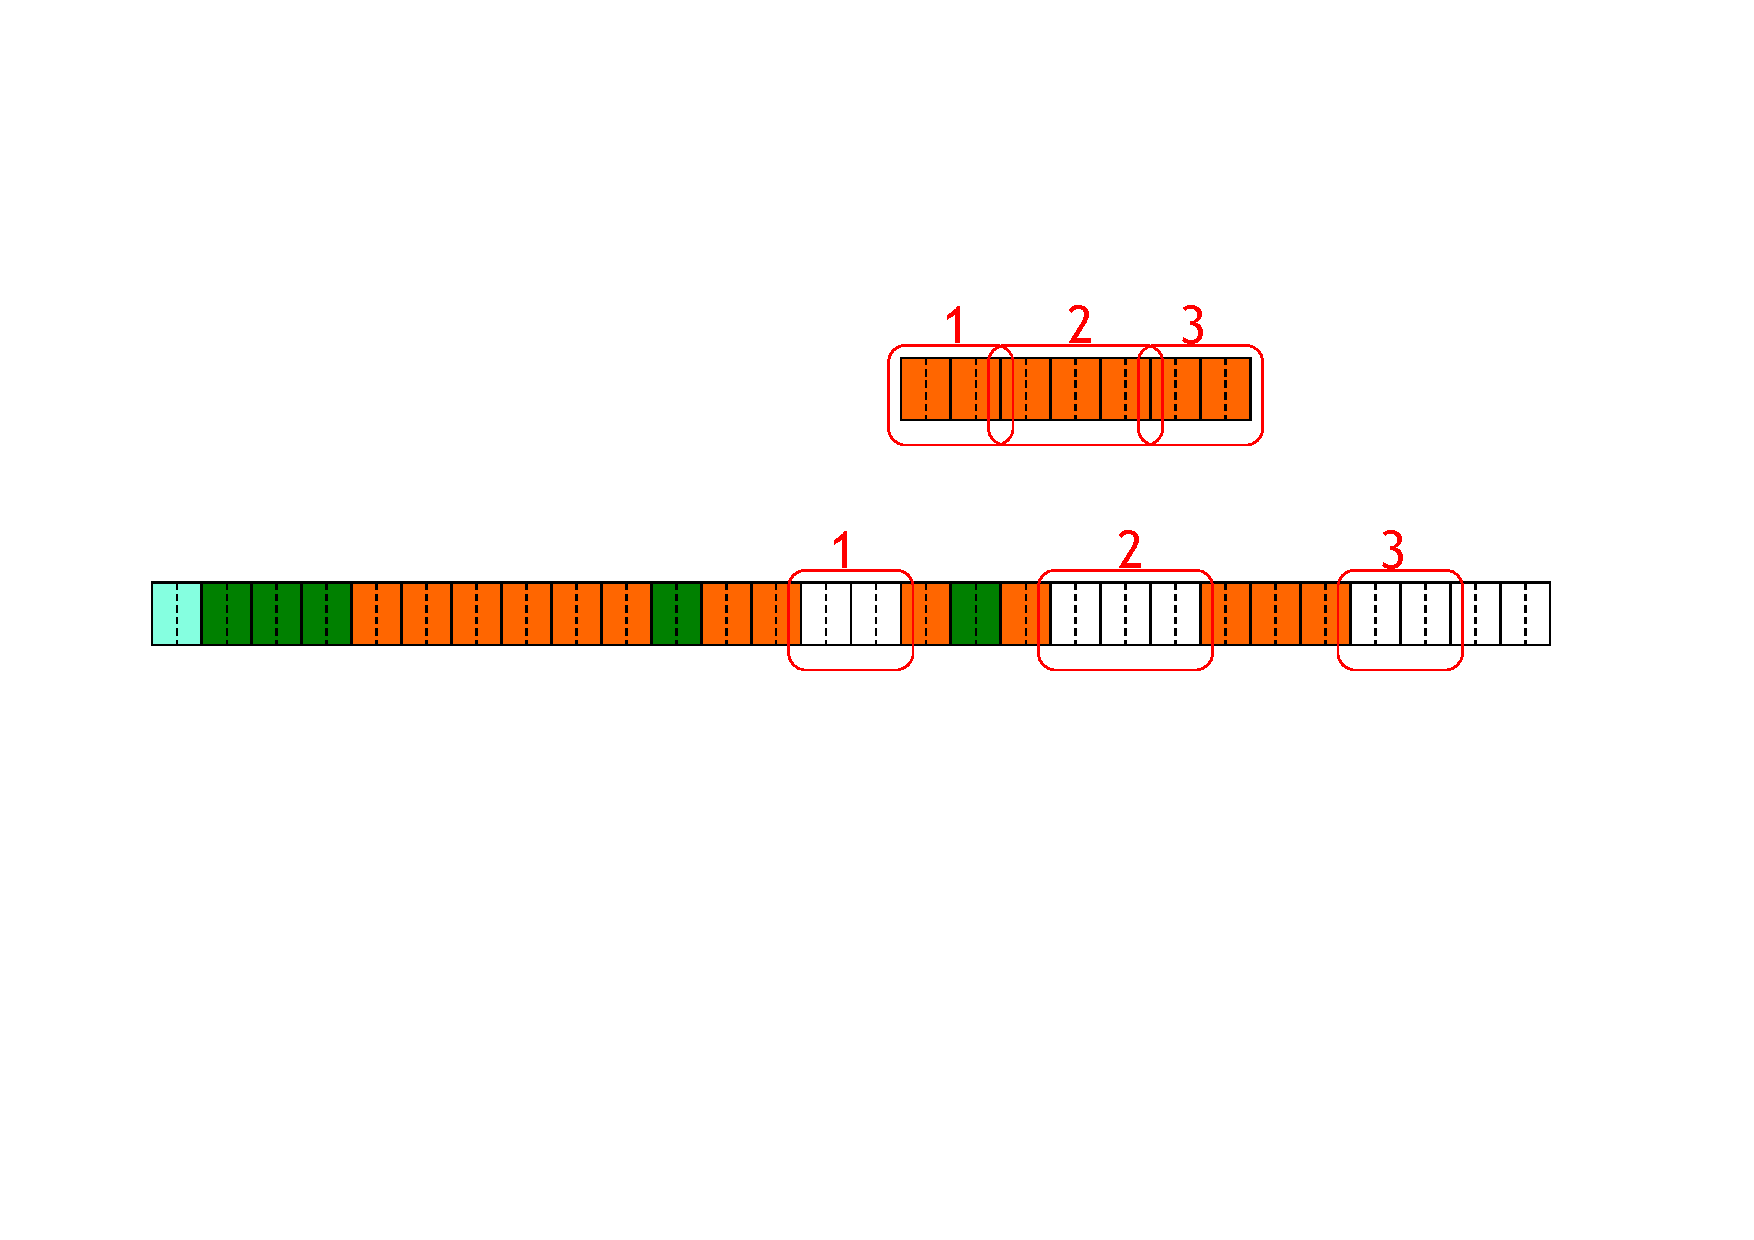
\includegraphics[width=\textwidth]{img/files-5.pdf}
    \end{figure}
\end{itemize}

\newpage

\paragraph{HDD}

\paragraph{SSD}

\paragraph{RAID}

\subsubsection{Networking (architecture and technology)}\label{subsubsection: Networking (architecture and technology)}
